

\section{Real-valued Function Optimization}

\begin{frame}{Real-valued Function Optimization}
  \begin{itemize}
    \item{Real-valued function}
      \begin{itemize}
        \item $f \colon \mathcal{S} \subset \mathbb{R}^n \to
          \mathbb{R},x \mapsto f(x)$
        \item $\mathcal{S} \colon $ search space
        \item Elements of $\mathcal{S} \colon $ candidates or solutions
      \end{itemize}
    \item{Optimization}
      \begin{itemize}
        \item $\mathop{\arg\min}\limits_{x} f(x)$, where $x$ are within given bounds.
        \item Maximizing $f$ is equivalent to minimizing $-f$.
      \end{itemize}
    \item Example
      \begin{itemize}
        \item $\mathop{\arg\min}\limits_x 2x^3-3x^2-36x-14$.
        \item Design of aircraft wings.
      \end{itemize}
  \end{itemize}
\end{frame}

\begin{frame}{Black-box Optimization}

  \begin{figure}[h]
    \includegraphics[scale=0.5]{BlackBox.eps}
    \caption{Black-box function}  
  \end{figure}
  \begin{itemize}
    \item The only information is the interaction between input and
    output.  
  \item The key point is investigating the trade-off between
    \alert{exploration}
    and \alert{exploitation}.
    \begin{itemize}
      \item Exploration is the capability of \alert{having an overview for the search
        space}.
  \item Exploitation is the capability of \alert{generating high resolution
    candidates}. 
    \end{itemize}
  \end{itemize}

\end{frame}

\begin{frame}{Difficulties}
  \begin{columns}
    \begin{column}{0.6\textwidth}
      \begin{itemize}[<+->]
        \item Non-convex
          \begin{itemize}
            \item Local optima are less important for global optimum.
          \end{itemize}
        \item Ruggedness
          \begin{itemize}  
            \item Perturbated by noise. 
            \item Non-smooth.
          \end{itemize}
        \item Dimensionality
          \begin{itemize}
            \item Search space grows exponentially
          \end{itemize}
        \item Non-separable
          \begin{itemize}
            \item Dependencies between decision variables
          \end{itemize}
        \item Ill-conditioned
          \begin{itemize}
            \item Unable to extract gradient information
          \end{itemize}
      \end{itemize}
    \end{column}
    \begin{column}{0.4\textwidth}
      \onslide<2->{
        \begin{figure}[l]
          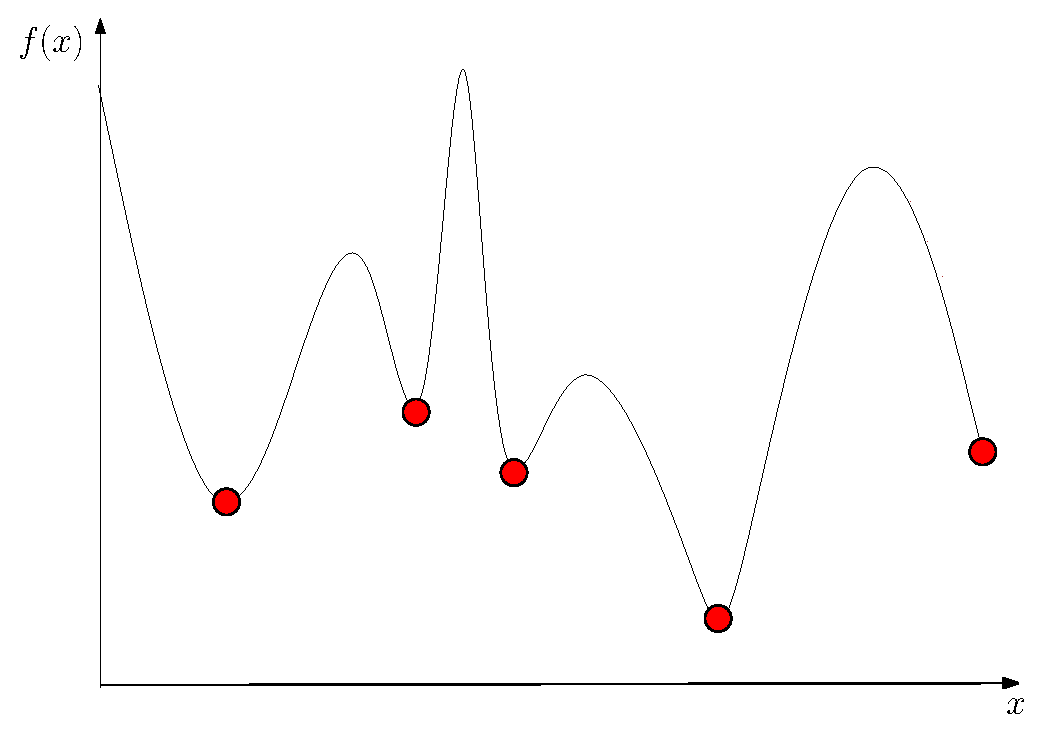
\includegraphics[width = 0.6\columnwidth]{Non-Convex.eps}
          \caption{Non-convex function}
        \end{figure}
      }
      \onslide<4->{
        \begin{figure}[H]
          \includegraphics[width = 0.6\columnwidth]{Rugged.eps}
          \caption{$sin(x)$ with noise}
        \end{figure}
      }
    \end{column}
  \end{columns}
\end{frame}
